\documentclass[12pt]{article}

\usepackage{fullpage}
\usepackage[spanish]{babel}
\usepackage{amsfonts} %for double trace letters
\usepackage{amssymb}
\usepackage{amsmath} %for special/unusual mathematical characters
\usepackage{eufrak} %for gothic letters
\usepackage{graphicx} %Image includer package
\graphicspath{{Images/}} %Image directory
\usepackage{xcolor}

\usepackage{multicol} %For writing text in columns
\setlength{\columnsep}{1cm} %Defines separation of columns

\usepackage{tcolorbox} %for boxes that enclose text
\usepackage{color}
\definecolor{myblue}{rgb}{.8, .8, 1}

\usepackage{empheq}

\newlength\mytemplen
\newsavebox\mytempbox

\makeatletter
\newcommand\mybluebox{%
    \@ifnextchar[%]
       {\@mybluebox}%
       {\@mybluebox[0pt]}}

\def\@mybluebox[#1]{%
    \@ifnextchar[%]
       {\@@mybluebox[#1]}%
       {\@@mybluebox[#1][0pt]}}

\def\@@mybluebox[#1][#2]#3{
    \sbox\mytempbox{#3}%
    \mytemplen\ht\mytempbox
    \advance\mytemplen #1\relax
    \ht\mytempbox\mytemplen
    \mytemplen\dp\mytempbox
    \advance\mytemplen #2\relax
    \dp\mytempbox\mytemplen
    \colorbox{myblue}{\hspace{1em}\usebox{\mytempbox}\hspace{1em}}}

% for theorems
\usepackage{amsthm}
 
\theoremstyle{definition}
\newtheorem{definition}{Definici\'on}[section]

\theoremstyle{theorem}
\newtheorem{theorem}{Teorema}[section]

% Defining my own math commands
\DeclareMathOperator{\Arg}{Arg}
\DeclareMathOperator{\Log}{Log}
\DeclareMathOperator{\sen}{sen}
\DeclareMathOperator{\senh}{senh}
\DeclareMathOperator{\tg}{tg}
\DeclareMathOperator{\ctg}{ctg}
\DeclareMathOperator{\tgh}{tgh}
\DeclareMathOperator{\ctgh}{ctgh}
\DeclareMathOperator{\sech}{sech}
\DeclareMathOperator{\csch}{csch}


\begin{document}
	\title{Funciones de Variable Compleja}
	\author{Breggia, Bruno M.}
	\date{}
	\maketitle
	

\begin{center}
	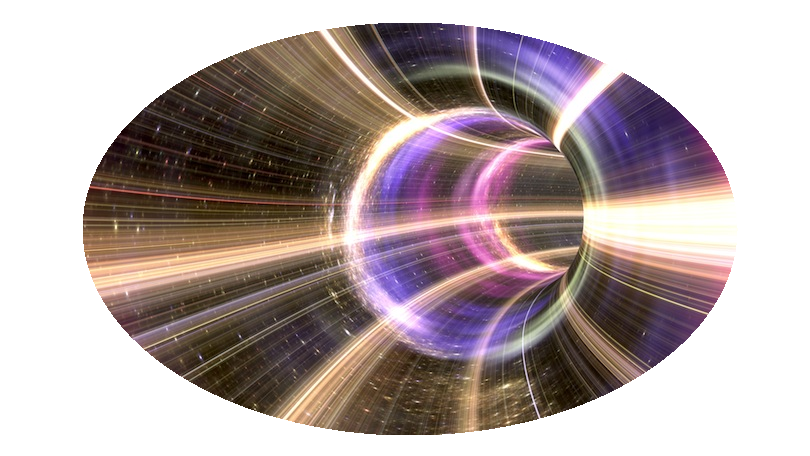
\includegraphics[scale=0.7]{wormwhole2.png}
\end{center}	
	
\begin{center}
\textit{``Comienza al principio, -dijo el rey, con voz grave-\\ y contin\'ua hasta que llegues al final, all\'i para"}
\end{center}

\begin{flushright}
Lewis Carroll, de \textbf{Alicia en el Pa\'is de las Maravillas}
\end{flushright}

Hemos llegado a un punto decisivo, la introducci\'on y definici\'on de las funciones de variable compleja, donde nos ser\'a revelado c\'omo, todo lo que conoc\'iamos hasta ahora de los n\'umeros reales no es m\'as que una \'infima porci\'on de lo que es el mundo detr\'as de escena del conjunto de los N\'umeros Complejos. Todas las funciones algebraicas elementales se generalizan de tal manera que cuando se les pasen valores reales, se comportan indistintamente a como lo hicieron siempre hasta el momento, pero con la diferencia de que ahora ser\'an capaces de recibir n\'umeros complejos, y el resultado de eso es algo jam\'as antes visto...

Prep\'arate para descononcer lo que sab\'ias hasta el momento, y conocer de cero lo que se viene. Bienvenido a \textbf{Variable Compleja.}

\pagebreak
\tableofcontents
\pagebreak

\section{Nos ponemos filos\'oficos: ?`Qu\'e es una funci\'on?}
Antes de entrar en detalle en lo que es una funci\'on de variable compleja, debemos recordar qu\'e es en s\'i mismo una funci\'on. Pareciese aburrido tener que retroceder a revisar un concepto tan elemental como lo es una \textit{funci\'on}, pero debemos tener en claro su definici\'on antes de generalizar el concepto.

Pero... ?`ser\'a tan f\'acil como parece? Def\'ineme \textit{funci\'on}... como si fuese obvio, he aqu\'i la definici\'on formal:\\

\colorbox{magenta!40!white!80}{\parbox{\linewidth}{
\theoremstyle{definition}
\begin{definition}{Funci\'on}

Una \textit{funci\'on} constituye una terna $(f, A, B)$, en donde:
\begin{itemize}
	\item $f$: es la \textbf{ley, regla o relaci\'on} que asigna a cada elemento del conjunto $A$ un \'unico elemento del conjunto $B$
	\item $A$: es el conjunto de partida, o \textbf{dominio}
	\item $B$: es el conjunto de llegada, o \textbf{codominio}
\end{itemize}
\end{definition}
}}
\linebreak
\linebreak

La notaci\'on simb\'olica de una funci\'on est\'a dada por
$$f:A\to B$$
$$f: x\in A \to y\ /\ y=f(x)\in B$$
Esto nos habilita a poder representar a la funci\'on $f$ evaluada para un valor $x\in A$ simplemente como $f(x)$, donde $f(x)\in B$, claro est\'a. Sin embargo, nunca deber\'iamos hablar de funciones sin antes especificar sus conjuntos de dominio y codominio (a menos que el contexto lo vuelva obvio). Tratemos que se vuelva costumbre.

\subsection{Caso especial: la Funci\'on Compleja}
Habiendo definido de manera gen\'erica lo que es una funci\'on, sabremos por intuici\'on que si nuestros conjuntos de dominio $A$ y codominio $B$ son ambos subconjuntos del conjunto de los n\'umeros reales, es decir: $A, B \in \mathbb{R}$, entonces tenemos definidas las funciones de una variable real. Cabe esperar entonces que para definir funciones de variable compleja debamos simplemente cambiar los conjuntos de partida y de llegada...\\

\colorbox{magenta!40!white!80}{\parbox{\linewidth}{
\theoremstyle{definition}
\begin{definition}{Funci\'on de Variable Compleja}

Una funci\'on compleja de variable compleja constituye una terna $(f, S, \mathbb{C}_w)$, en donde:
\begin{itemize}
	\item $f$: \textbf{ley, regla o relaci\'on} que asigna a cada elemento de $S$ un \'unico elemento en $\mathbb{C}_w$
	\item $S$: es el conjunto \textbf{dominio} de $f$, con $f\subset \mathbb{C}_z$
	\item $\mathbb{C}_w$: es el conjunto \textbf{codominio} de $f$
\end{itemize}
\end{definition}
}}
\linebreak
\linebreak

Para terminar con el precalentamiento, vale diferenciar entre los distintos tipos de funciones complejas, ya que de tanto en tanto, utilizaremos funciones que mapeen variables complejas a n\'umeros complejos, como funciones que mapeen variables \textit{reales} a n\'umeros complejos.

\begin{itemize}
	\item \textbf{Funciones de Variable Compleja a valores complejos}: son las funciones dadas por $f:S\subset \mathbb{C}_z \to D\in \mathbb{C}_w$, que reciben un n\'umero complejo $z\in S$, con $z=x+iy$, y retornan otro complejo $w=f(z)\in D$, donde diremos que $w = u+iv$. Este tipo de funciones pueden escribirse de la forma:

	\begin{empheq}[box={\mybluebox[5pt]}]{equation*}
		\mbox{ $w=f(z)=u(x,y)+i\ v(x,y)$ }
	\end{empheq}	
	
	 ...ya que tanto la parte real como imaginaria de la funci\'on dependen de la parte real e imaginaria de la variable que recibe (?`de qu\'e m\'as puede depender?). Si prestan particular atenci\'on, tanto $u(x,y)$ como $v(x,y)$ son ambas funciones de \textit{dos} variables reales, que retornan un valor real, es decir, $u,v : \tilde{S} \in \mathbb{R}^2\to \mathbb{R}$.
	
	Los conjuntos de partida $\tilde{S}\in \mathbb{R}^2$ y $S\in \mathbb{C}$ tienen una correspondencia biun\'ivoca (y los de llegada tambi\'en).
	
	\item \textbf{Funciones de Variable Real a valores complejos}: son las funciones dadas por $f: I = (a,b)\in \mathbb{R} \to \mathbb{C}$. En \'estos, se recibe una variable real $t\in I$, y se obtiene un n\'umero complejo $z = f(t) = x+iy$. Si recordamos la relaci\'on biun\'ivoca entre $\mathbb{C}$ y $\mathbb{R}^2$, y la representaci\'on gr\'afica de n\'umeros complejos, concluimos entonces que este tipo de funciones son como parametrizaciones, en donde tendremos un complejo diferente a medida que recorramos el intervalo real $[a,b]$.
	
	Para que quede m\'as claro, representemos a la funci\'on de la siguiente manera:
	\begin{empheq}[box={\mybluebox[5pt]}]{equation*}
		\mbox{ $z(t)=f(t)= u(t) + i\ v(t)$ }
	\end{empheq}
	
	 ...en donde $u,v : I=(a,b)\in \mathbb{R}\to \mathbb{R}$, es decir, $u,v$ son dos funciones de una variable real a valores reales.
\end{itemize}

Al fin y al cabo, toda funci\'on compleja puede desglosarse en t\'erminos de funciones de una o m\'as variables \textit{reales}, con las cuales ya somos h\'abiles manipulando.

\section{A trav\'es del espejo}
Procederemos a analizar ahora la extensi\'on de la definici\'on de todas la funciones algebraicas elementales de tal manera que acepten n\'umeros complejos como par\'ametros... !`y a sorprenderse con lo que obtengamos de ellas!\\

\colorbox{red!40!white!80}{\parbox{\linewidth}{
\theoremstyle{definition}
\begin{definition}{Funci\'on exponencial Compleja}

La funci\'on exponencial compleja $\exp(z) = e^{z}$ se define, a trav\'es de la f\'ormula de Euler, como: $$\exp(z) = e^z = e^{x+iy} \triangleq e^x(\cos y + i\sen y)$$

\end{definition}
}}
\linebreak
\linebreak

Dados $z, z_1, z_2 \in \mathbb{C}$, reconocemos las siguientes propiedades de la exponencial compleja:
\begin{enumerate}
	\item $e^z \neq 0,\ \forall z \in \mathbb{C}$ (puede tomar valores negativos)
	\item $e^z = e^x$ si $z$ es un real puro (con parte imaginaria 0)
	\item $e^{z_1+z_2} = e^{z_1}e^{z_2}$
	\item $|e^z| = e^x$
	\item $(e^z)^n = e^{nz},\ \forall n \in \mathbb{Z}$
	\item $\arg(e^z) = y + 2k\pi,\ \forall k \in \mathbb{Z}$
	\item $e^z = e^{z + 2\pi i}$, por lo que es una funci\'on peri\'odica con periodo $2\pi i$	
\end{enumerate}

Si quisi\'esemos representar a la funci\'on exponencial compleja en la forma $f(z) = u(x, y) + i\cdot v(x, y)$, tendr\'iamos lo siguiente:
$$e^z = \exp z = (e^x \cos y) + i\ (e^x \sen y)$$\\

\colorbox{red!40!white!80}{\parbox{\linewidth}{
\theoremstyle{definition}
\begin{definition}{Funciones Trigonom\'etricas Complejas}

Las funciones trigonom\'etricas complejas del seno y coseno se definen como sigue, en t\'erminos de la exponencial compleja:
\begin{center}
	\begin{tabular}{ccc}
		$\displaystyle \cos z \triangleq \frac{e^{iz} + e^{-iz}}{2} $ &\ \ & $\displaystyle \sen z \triangleq \frac{e^{iz} - e^{-iz}}{2i} $\\
	\end{tabular}
\end{center}
\end{definition}
}}
\linebreak
\linebreak

Dados $z, z_1, z_2 \in \mathbb{C}$, reconocemos las siguientes propiedades del coseno y seno complejos:
\begin{enumerate}
	\item $\cos z = \cos x\ \land\ \sen z = \sen x$, si $z$ es un real puro (con parte imaginaria 0)
	\item $\cos(-z) = \cos {z}\ \land\ \sen(-z) = -\sen z$
	\item $\sen^2 z + \cos^2 z = 1$
	\item $\sen(z_1 \pm z_2) = \sen z_1 \cos z_2 \pm \cos z_1 \sen z_2$
	\item $\cos(z_1 \pm z_2) = \cos z_1 \cos z_2 \mp \sen z_1 \sen z_2$
\end{enumerate}

A partir de las definiciones del coseno y seno de n\'umeros complejos, definimos de manera m\'as sencilla las dem\'as funciones trigonom\'etricas:

\begin{center}
	\begin{tabular}{cccc}
	$\displaystyle \tg z = \frac{\sen z}{\cos z} $ & $\displaystyle \ctg z = \frac{\cos z}{\sen z} $ & $\displaystyle \csc z = \frac{1}{\sen z} $ & $\displaystyle \sec z = \frac{1}{\cos z} $ \\
	\end{tabular}
\end{center}

Si quisi\'esemos representar a la funci\'on coseno y seno complejos en la forma $f(z) = u(x, y) + i\cdot v(x, y)$, luego de cierto trabajo algebraico, llegar\'iamos a lo siguiente:
$$\cos z = \cos(x + iy) = \cos x \cosh y + i\sen x \senh y$$
$$\sen z = \sen(x + iy) = \sen x \cosh y + i\cos x \senh y$$\\

\colorbox{red!40!white!80}{\parbox{\linewidth}{
\theoremstyle{definition}
\begin{definition}{Funciones Hiperb\'olicas Complejas}

Se definen las funciones hiperb\'olicas complejas coseno hiperb\'olico y seno hiperb\'olico a partir de la funci\'on exponencial compleja:
\begin{center}
	\begin{tabular}{ccc}
		$\displaystyle \cosh z \triangleq \frac{e^{z} + e^{-z}}{2} $ &\ \ & $\displaystyle \senh z \triangleq \frac{e^{z} - e^{-z}}{2} $\\
	\end{tabular}
\end{center}
\end{definition}
}}
\linebreak
\linebreak

Dados $z, z_1, z_2 \in \mathbb{C}$, reconocemos las siguientes propiedades del coseno y seno hiperb\'olicos complejos:
\begin{enumerate}
	\item $\cosh z = \cosh x\ \land\ \senh z = \senh x$, si $z$ es un real puro (con parte imaginaria 0)
	\item $\cosh (-z) = \cosh z\ \land\ \senh(-z) = -\senh z$
	\item $\cosh^2 z - \senh^2 z = 1$
	\item $\senh(z_1 \pm z_2) = \senh z_1 \cosh z_2 \pm \cosh z_1 \senh z_2$
	\item $\cosh(z_1 \pm z_2) = \cosh z_1 \cosh z_2 \pm \senh z_1 \senh z_2$
\end{enumerate}

A partir de las definiciones del coseno y seno hiperb\'olicos de n\'umeros complejos, definimos de manera m\'as sencilla las dem\'as funciones hiperb\'olicas:

\begin{center}
	\begin{tabular}{cccc}
	$\displaystyle \tgh z = \frac{\senh z}{\cosh z} $ & $\displaystyle \ctgh z = \frac{\cosh z}{\senh z} $ & $\displaystyle \csch z = \frac{1}{\senh z} $ & $\displaystyle \sech z = \frac{1}{\cosh z} $ \\
	\end{tabular}
\end{center}

Si quisi\'esemos representar a las funciones coseno y seno hiperb\'olicas complejas en la forma $f(z) = u(x, y) + i\cdot v(x, y)$, luego de cierto trabajo algebraico, llegar\'iamos a lo siguiente:
$$\cosh z = \cosh(x + iy) = \cosh x \cos y + i\senh x \sen y$$
$$\senh z = \senh(x + iy) = \senh x \cos y + i\cosh x \sen y$$

Como podemos apreciar, las funciones trigonom\'etricas y las hiperb\'olicas no s\'olo poseen abismales similitudes entre s\'i, sino que tambi\'en guardan una relaci\'on mutua que puede ser descubierta una vez adentrados en variable compleja. Miremos unas propiedades m\'as que las involucran:
\begin{itemize}
	\item $\sen(iz) = i\cdot \senh z\ \land\ \cos(iz) = \cosh z$
	\item $\senh(iz) = i\cdot \sen z\ \land\ \cosh(iz) = \cos z$
	\item $|\sen z|^2 = \sen^2 x + \senh^2 y \ \land\ |\cos z|^2 = \cos^2 x + \cosh^2 y$
	\item $|\senh z|^2 = \senh^2 x + \sen^2 y\ \land\ |\cosh z|^2 = \cosh^2 x + \cos^2 y$
\end{itemize}
\ \\

\colorbox{red!40!white!80}{\parbox{\linewidth}{
\theoremstyle{definition}
\begin{definition}{Funci\'on Logaritmo Complejo}

Se define el logaritmo de un n\'umero complejo $z\neq 0$ como:
\begin{eqnarray*}
\log z &\triangleq& \ln |z| + i \cdot \arg z \\
&=& \ln |z| + i \cdot (\Arg z + 2k\pi),\ k \in \mathbb{Z}
\end{eqnarray*}
Para distintos $k$ tendremos un valor distinto de logaritmo. Esto contradice en cierto sentido a la definici\'on de funci\'on, ya que tenemos aqu\'i una relaci\'on \textbf{multivaluada}: para cada valor del dominio, resulta ser que tenemos m\'as de un elemeto en el codominio que cumple con la ley aplicada. Es por ello que tratamos de enmendar este imprevisto definiendo alternativamente el \textbf{Logaritmo univaluado}:
$$\Log z \triangleq \ln |z| + i\cdot \Arg z$$

\end{definition}}}
\linebreak
\linebreak

Dados $z, z_1, z_2 \in \mathbb{C}$, reconocemos las siguientes propiedades del logaritmo complejo:
\begin{enumerate}
	\item $\log (z_1z_2) = \log z_1 + \log z_2$
	\item $\displaystyle\log \frac{z_1}{z_2} = \log z_1 - \log z_2$
	\item $\log z^n = n\cdot \log z,\ n \in \mathbb{Z}$
\end{enumerate}

Ya dada la definici\'on del logaritmo complejo, podemos apreciar c\'omo \'esta es la inversa de la funci\'on exponencial. Sea $w = \log z$, con $z \neq 0$, entonces $z=e^w$, y a partir de ello...
\begin{eqnarray*}
z &=& |z|\ e^{i \arg z}\\
z &=& |z|\ e^{i\ (\Arg z + 2k\pi)}\\
z &=& e^u \cdot e^{iv} = e^{u+iv}
\end{eqnarray*}
... con $u = \ln |z|$ y con $v = \Arg z + 2k\pi$ (esto es, con el logaritmo natural $\ln$ definido \'unicamente para los reales positivos y con $k \in \mathbb{Z}$). Pero como $z = e^w$:
\begin{eqnarray*}
e^w &=& e^{u+iv}\\
w &=& u+iv\\
w &=& \ln |z| + i(\Arg z + 2k\pi)
\end{eqnarray*}

\section{Nos vamos al L\'imite}
?`Pensaban que con ver un par de funciones complejas acababa todo? Pues si nos tomamos el trabajo de estudiarlas, que no sea en vano. Ya que se vieron algunas funciones complejas, pasemos de largo y continuemos redefiniendo conceptos del c\'alculo en variable real de tal manera que engloben a las variables complejas. Si nos detuvi\'esemos aqu\'i, nos perder\'iamos de lo mejor.\\

\colorbox{yellow!40!white!80}{\parbox{\linewidth}{
\theoremstyle{definition}
\begin{definition}{L\'imites de funciones complejas}

Sea $f: S \subset \mathbb{C} \rightarrow \mathbb{C}$. Se dice que el l\'imite de una funci\'on $f$ cuando $z$ tiende a un valor $z_0$ es igual a $w_0$ y se indica:
$$\lim\limits _{z\rightarrow z_0} f(z) = w_0$$
si el valor de $f(z)$ se hace cada vez m\'as cercano a $w_0$ conforme $z$ se va acercando indefinidamente a $z_0$, pero sin igualarlo.

En lenguaje simb\'olico (con $\varepsilon, \delta \in \mathbb{R}$), se tiene que el l\'imite de $f(z)$ conforme $z \rightarrow z_0$ es $w_0$ si y s\'olo si:
$$\forall \varepsilon >0, \exists \delta > 0\ /\ \forall z \in \eta^*(z_0, \delta) \Rightarrow f(z) \in \eta(w_0, \varepsilon)$$

O tambi\'en si:
$$\forall \varepsilon >0, \exists \delta > 0\ /\ 0<|z-z_0|<\delta \Rightarrow |f(z)-w_0|<\varepsilon$$

\end{definition}}}
\linebreak
\linebreak

\colorbox{orange!40!white!80}{\parbox{\linewidth}{
\theoremstyle{theorem}
\begin{theorem}{Unicidad del l\'imite}

Sea $f: S \subset \mathbb{C} \rightarrow \mathbb{C}$. Para $z_0 \in \mathbb{C}$ y $z$ una variable compleja, si el l\'imite $$\lim\limits_{z\rightarrow z_0} f(z)$$
existe, entonces es \'unico.
\end{theorem}}}
\linebreak

Demostrar
\linebreak

\colorbox{orange!40!white!80}{\parbox{\linewidth}{
\theoremstyle{theorem}
\begin{theorem}

Sea $f: S \subset \mathbb{C} \rightarrow \mathbb{C}$. Teniendo que $f(z) = u(x, y) + i\cdot v(x, y)$ y $z_0, w_0 \in \mathbb{C}$ con $z_0 = x_0 + iy_0$ y $w = u_0+iv_0$, entonces:
$$\lim\limits_{z\rightarrow z_0} f(z) = w_0 \Leftrightarrow \lim\limits_{(x, y)\rightarrow (x_0, y_0)}u(x,y) = u_0\ \land\ \lim \limits_{(x, y)\rightarrow (x_0, y_0)}v(x,y) = v_0$$
\end{theorem}}}
\linebreak

Demostrar\\

Propiedades de los l\'imites: dado que los l\'imites $\lim\limits_{z\rightarrow z_0} f(z) = w_1$ y $\lim\limits_{z\rightarrow z_0} g(z) = w_2$ existan, se cumple que...
\begin{enumerate}
	\item $\lim\limits_{z\rightarrow z_0} [f(z) + g(z)] = w_1 + w_2$
	\item $\lim\limits_{z\rightarrow z_0} [f(z) \cdot g(z)] = w_1 \cdot w_2$
	\item $\displaystyle \lim\limits_{z\rightarrow z_0} \frac{f(z)}{g(z)} = \frac{w_1}{w_2}$, siempre que $w_2 \neq 0$
\end{enumerate}

\section{El Infinito en un punto}
Hay situaciones que surgen en donde se nos es necesario poder representar, de alguna manera, el infinito. Hablo de representarlo como un n\'umero en concreto, al que tienden los l\'imites en el m\'as all\'a, o como un punto, el punto donde se cortan dos rectas paralelas... Cuando tratamos con el conjunto de los n\'umeros complejos, suele surgir esta necesidad. Por esto mismo es que definimos el \textbf{Punto Infinito}.\\

\colorbox{blue!40!white!80}{\parbox{\linewidth}{
\theoremstyle{definition}
\begin{definition}{El Punto Infinito}

El n\'umero complejo infinito, o \textbf{punto infinito}, denotado por $\infty$, es un \'unico n\'umero complejo, para el cual el plano complejo no admite representaci\'on gr\'afica.

Podemos considerar a $\infty$ como un n\'umero complejo cuyo m\'odulo es mayor que cualquier n\'umero real positivo dado, pero sin argumento.

\end{definition}}}
\linebreak
\linebreak

Es en base a todo esto, definiremos como consecuencia al \textbf{conjunto complejo extendido} $\mathbb{C}^\infty$ como:
$$\mathbb{C}^\infty = \mathbb{C} \cup \{\infty\}$$

\section{Cotinuemos con Continuidad}
Hemos definido l\'imites de funciones de variables complejas, ahora, de qu\'e tanta utilidad nos ser\'ia el l\'imite si no fuese para definir, entre otras cosas, algo tan elemental como ser la continuidad del trazo de una funci\'on. Eso es, me refiero a la definici\'on de continuidad, !`aplicado a funciones de variable compleja!\\


\colorbox{green!40!white!80}{\parbox{\linewidth}{
\theoremstyle{definition}
\begin{definition} {Continuidad}

Sea $f: S \subset \mathbb{C} \rightarrow \mathbb{C}$ y $z_0 \in S$. Se dice que $f(z)$ es \textbf{continua} en $z_0$ si satisface:
\begin{itemize}
	\item $\exists \lim\limits_{z\rightarrow z_0}f(z)$
	\item $\exists f(z_0)$
	\item $\lim\limits_{z\rightarrow z_0}f(z) = f(z_0)$
\end{itemize}

\end{definition}}}
\linebreak
\linebreak

\colorbox{green!40!white!80}{\parbox{\linewidth}{
\theoremstyle{definition}
\begin{definition} {Continuidad sobre un conjunto $S$}

Sea $f: S \subset \mathbb{C} \rightarrow \mathbb{C}$\\
Diremos que $f$ es \textbf{continua en $S$} si es continua en todo $z \in S$.
\end{definition}}}
\linebreak
\linebreak

\colorbox{green!40!white!80}{\parbox{\linewidth}{
\theoremstyle{definition}
\begin{definition} {Funci\'on acotada}

Sea $f: S \subset \mathbb{C} \rightarrow \mathbb{C}$\\
Diremos que $f$ es una \textbf{funci\'on acotada} si $\exists M \in \mathbb{R}^+$ tal que $|f(z)| \leq M,\ \forall z \in S$.
\end{definition}}}
\linebreak
\linebreak

En base a estas definiciones, se desprende el siguiente, e intuitivo, teorema.\\

\colorbox{orange!40!white!80}{\parbox{\linewidth}{
\theoremstyle{theorem}
\begin{theorem} {Continuidad y acotaci\'on}

Sea $f: S \subset \mathbb{C} \rightarrow \mathbb{C}$\\
Si $S$ es un conjunto compacto y $f(z)$ es una funci\'on continua en $S$, entonces $f$ es una funci\'on acotada.
\end{theorem}}}
\linebreak
\linebreak

\end{document}